\documentclass[10pt,a4paper]{article}
\usepackage[utf8]{inputenc}
\usepackage[T1]{fontenc}
\usepackage[spanish,es-noshorthands,es-nodecimaldot,es-tabla]{babel}
\usepackage{lmodern}
\usepackage[margin=1.55cm,top=1.4cm,bottom=1.6cm]{geometry}
\usepackage{amsmath,amssymb,mathtools}
\usepackage{graphicx}
\usepackage{booktabs}
\usepackage[font=small,labelfont=bf,skip=2pt]{caption}
\usepackage{subcaption}
\usepackage{microtype}
\usepackage{xcolor}
\usepackage[colorlinks=true,linkcolor=blue!50!black,urlcolor=blue!50!black]{hyperref}

\graphicspath{{../tarea3_param/experimentos/resultados/}}
\setlength{\parindent}{0pt}
\setlength{\parskip}{2.5pt}
\setlength{\textfloatsep}{6pt plus 2pt minus 2pt}
\setlength{\floatsep}{5pt plus 2pt minus 2pt}
\setlength{\intextsep}{5pt plus 2pt minus 2pt}
\renewcommand{\arraystretch}{0.95}
\setcounter{topnumber}{3}
\renewcommand{\topfraction}{0.85}
\renewcommand{\textfraction}{0.1}
\renewcommand{\floatpagefraction}{0.8}

\newcommand{\code}[1]{\texttt{#1}}
\newcommand{\preg}[1]{\textbf{#1}\enspace}
\newcommand{\seccion}[1]{\vspace{3pt}{\large\bfseries #1}\par\vspace{1pt}}

\begin{document}

\begin{center}
{\LARGE\bfseries Tarea 3: Parametrización de superficies}\\[2pt]
{\large CC5513 -- Procesamiento Geométrico y Análisis de Formas}\\[2pt]
Matías Saavedra \quad·\quad Informe
\end{center}
\suppressfloats[t]

\seccion{Implementación}
\textbf{Pesos (Parte 1).} Ambas funciones recorren las 3 esquinas de los triángulos (el único ciclo) y generan tripletas $(i,j,w)$ que \code{\_sparse\_from\_triplets} suma. En \code{cotangent\_weights}, el ángulo $\theta_c$ de la esquina $c$ (\code{corner\_angles}) es opuesto a la arista $(a,b)=(F_{c+1},F_{c+2})$, y se agrega $\tfrac12\cot\theta_c$ a $W[a,b]$ y a $W[b,a]$: una arista interior acumula $\tfrac12(\cot\alpha+\cot\beta)$ y una de borde un solo término. En \code{mean\_value\_weights}, el ángulo $\gamma$ en $v_i=F_c$ aporta $\tan(\gamma/2)/\|v_i-v_j\|$ a $W[i,j]$ para los dos lados del triángulo que salen de $v_i$, así que las dos caras de una arista suman $\tan(\gamma/2)+\tan(\delta/2)$ (matriz no simétrica). En Lucy tardan unos 0.02\,s (el límite es 1\,s) y coinciden con una implementación de referencia arista por arista (diferencia $<10^{-14}$).
\textbf{Borde poligonal (Parte 2).} \code{polygon\_points} cierra el polígono, calcula la distancia acumulada desde \code{corners[0]} hasta cada esquina, convierte $t$ en $s=(t \bmod 1)P$ e interpola $x$ e $y$ linealmente entre esquinas con \code{np.interp} (que hace la búsqueda de \code{searchsorted}); así el perímetro se recorre a velocidad constante.
\textbf{Pruebas y experimentos.} \code{python tests.py} pasa 12/12 pruebas (agregamos tres: valores exactos en un abanico regular, un rectángulo con $t=1$ y el bonus B1). Cada parte tiene un script en \code{tarea3\_param/experimentos/} que genera sus figuras y tablas (Anexo~\ref{anx:reproduccion}).

\seccion{Parte 1. Pesos armónicos y de valor medio}
\begin{table}[h]
\centering\small
\caption{Pesos cotangentes negativos y triángulos invertidos con borde circular.}
\label{tab:p1}
\begin{tabular}{lrrrrr}
\toprule
malla & \code{neg\_w} (aristas) & interiores con $\alpha+\beta>\pi$ & de borde con $\alpha>\pi/2$ & triáng.\ obtusos & flips (armónico, círculo) \\
\midrule
Nefertiti & 86 (43) & 35 & 8 & 27\,\% & 0 \\
Bunny & 922 (461) & 459 & 2 & 42\,\% & 0 \\
Lucy & 11\,192 (5\,596) & 5\,565 & 31 & 48\,\% & 1 \\
\bottomrule
\end{tabular}
\end{table}

\preg{1.1} \code{neg\_w} es 86 en Nefertiti, 922 en Bunny y 11\,192 en Lucy (Tabla~\ref{tab:p1}). Cuenta entradas de $W$, y como $W$ es simétrica son 43, 461 y 5\,596 aristas. Como $\cot\alpha+\cot\beta=\sin(\alpha+\beta)/(\sin\alpha\sin\beta)$ y $\sin\alpha,\sin\beta>0$, se tiene $D_{ij}<0 \iff \alpha+\beta>\pi$ (la arista no es localmente Delaunay); en una arista de borde, $D_{ij}<0\iff\alpha>\pi/2$. La tabla confirma que las aristas negativas son exactamente esas. Con pesos negativos \emph{no} se cumple la hipótesis del teorema: $u_i$ deja de ser combinación convexa de sus vecinos y puede salir de su envoltura convexa, así que no hay garantía de biyectividad. Con borde circular (tres mallas, dos espaciados) aparece un único triángulo invertido: Lucy, cara 18\,885, con ángulos de 46, 118.5 y 15 grados (Fig.~\ref{fig:p12}a, modo \code{flips}: rojo = \code{per\_face["flipped"]}). En $(u,v)$ queda como una astilla 150 veces más larga que alta, que no se alcanza a ver en el visor, y en 3D ya está plegada: su normal forma 159--174 grados con las de sus tres vecinas. Los pesos cotangentes, que siguen la geometría, reproducen ese pliegue (LSCM, con el mismo Laplaciano, también); los de valor medio dejan la cara bien orientada.

\preg{1.2} En un triángulo no degenerado los ángulos en $v_i$ cumplen $0<\gamma,\delta<\pi$, luego $\gamma/2,\delta/2\in(0,\pi/2)$ y sus tangentes son positivas; además $\|v_i-v_j\|>0$. Por lo tanto $D_{ij}>0$ siempre (también con un solo término), sin importar la forma de los triángulos ni si el anillo es plano (mínimos medidos: 0.12, 3.67 y 5.01). Esto garantiza que cada vértice interior es combinación convexa estricta de sus vecinos ($\lambda_{ij}=D_{ij}/\sum_kD_{ik}>0$), que $L_{II}$ es invertible (M-matriz) y, por Tutte--Floater, que con un borde convexo la parametrización es biyectiva para cualquier malla; el teorema solo necesita filas convexas, no simetría. En Lucy, valor medio + círculo no tiene flips.

\preg{1.3} Si la malla es plana y el borde se fija en su posición original, las coordenadas originales $x$ resuelven $LU=0$ si y solo si $\sum_jD_{ij}(x_j-x_i)=0$ en cada vértice interior, y como la solución es única se recuperan exactamente. Los pesos cotangentes lo cumplen porque $\sum_jD_{ij}(x_i-x_j)=\partial E_D/\partial x_i$, la derivada de la energía de Dirichlet de la función lineal a trozos: para $x$ lineal $\nabla x$ es constante, y $\partial E_D/\partial x_i=\nabla x\cdot\int\nabla\varphi_i\,dA=0$ porque la función sombrero $\varphi_i$ de un vértice interior se anula en el borde de su estrella. Los de valor medio están construidos justamente para reproducir funciones lineales (Floater los obtiene de la propiedad del valor medio de las funciones armónicas, aplicada a $x$). Los uniformes exigen que $x_i$ sea el centroide de sus vecinos, falso en una malla irregular: en la malla plana el error es $2.5\cdot10^{-2}$ y \code{conf\_med} 1.533, frente a $5\cdot10^{-14}$ (cotangentes) y $10^{-15}$ (valor medio) con \code{conf\_med} 1.000. Consecuencia práctica: en zonas casi planas los pesos cotangentes y de valor medio conservan la forma de los triángulos (el mapa es localmente casi una semejanza), mientras que Tutte ``regulariza'' la malla y la distorsiona según el muestreo y no según la geometría. En el 25\,\% de caras menos curvas (menor defecto angular), \code{conf\_med} es 1.44/1.90/1.89 con pesos uniformes y 1.13/1.29/1.25 con cotangentes (Nefertiti/Bunny/Lucy).

\begin{figure}[t]
\centering
\begin{subfigure}[t]{0.3\textwidth}\centering
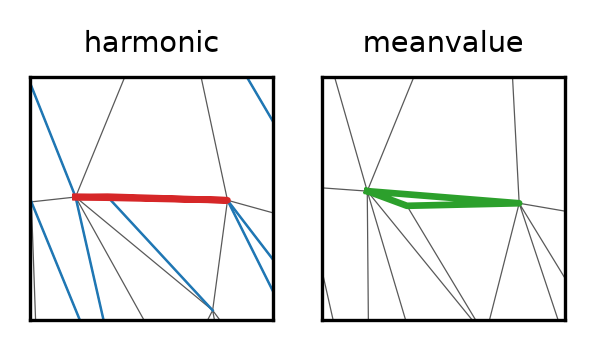
\includegraphics[width=\linewidth]{p1_lucy_flip_uv.png}
\caption{Lucy, círculo: la cara 18\,885 queda invertida con pesos armónicos (rojo) y no con valor medio (verde); azul: $D_{ij}<0$.}
\end{subfigure}\hfill
\begin{subfigure}[t]{0.3\textwidth}\centering
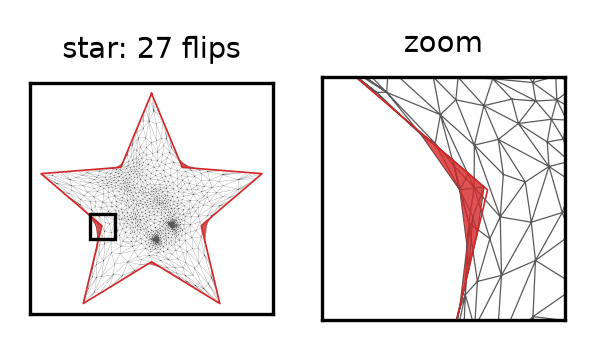
\includegraphics[width=\linewidth]{p2_bunny_estrella_uv.png}
\caption{Bunny, valor medio + estrella.}
\end{subfigure}\hfill
\begin{subfigure}[t]{0.37\textwidth}\centering
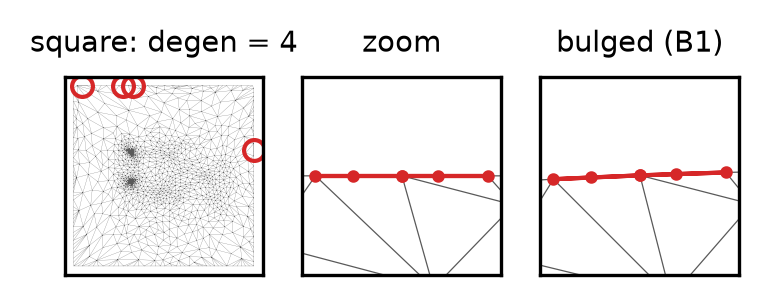
\includegraphics[width=\linewidth]{p2_bunny_orejas_uv.png}
\caption{Bunny, valor medio + cuadrado: las 4 caras degeneradas (círculos), zoom de dos y el mismo zoom con el borde del bonus B1.}
\end{subfigure}
\caption{Caras invertidas (rojo, el mismo arreglo que pinta el modo \code{flips}) y degeneradas en el dominio $(u,v)$.}
\label{fig:p12}
\end{figure}

\seccion{Parte 2. Bordes poligonales}
\preg{2.1} Las 4 caras degeneradas de Bunny son ``orejas'' del borde: triángulos con sus 3 vértices consecutivos en el borde (posiciones 23--25, 58--60, 60--62 y 67--69, en el contorno de la base). El vértice del medio tiene solo esos dos vecinos y la arista que une los otros dos es interior con ambos extremos en el borde (``arista divisoria''). Con el cuadrado los tres caen en el mismo lado, quedan colineales y el área es 0 (Fig.~\ref{fig:p12}c); como la cara queda determinada por el borde, pasa con los tres pesos y los dos espaciados. En un círculo tres puntos distintos nunca son colineales. No contradice el teorema: este vale para bordes estrictamente convexos; con un polígono de lados rectos, la versión precisa (Floater 2003) exige que ninguna arista divisoria quede sobre un lado, y la de Tutte un grafo 3-conexo, que falla en un vértice de grado 2. Además la cara es degenerada pero no invertida. Para evitarlo: usar una curva estrictamente convexa (círculo o el cuadrado abombado del bonus B1); poner una esquina del cuadrado en el vértice del medio de cada oreja (sirve en Bunny, con 4 orejas, no en Lucy, con 21); o preprocesar la malla volteando o dividiendo las aristas divisorias.

\preg{2.2} La estrella no es convexa, así que el teorema no aplica aunque los pesos sean positivos. Con pesos positivos cada vértice interior queda en la envoltura convexa de sus vecinos, y cerca de un vértice cóncavo del borde esa envoltura sale de la estrella: los triángulos de esa zona se pliegan sobre el borde (Fig.~\ref{fig:p12}b). Con espaciado \code{arc} hay 13/12/14 flips en Nefertiti, 41/28/27 en Bunny y 272/238/158 en Lucy (uniforme/armónico/valor medio), y el 93--100\,\% están a menos de 0.2 de uno de los 5 vértices cóncavos; ninguno cerca de las puntas convexas.

\begin{table}[h]
\centering\small
\caption{Espaciado \code{arc} $\to$ \code{uniform} (pesos armónicos, círculo). ``Borde'': caras que tocan el borde.}
\label{tab:arc}
\begin{tabular}{lrcccccc}
\toprule
malla & $n_b$ & cv / máx:mín aristas del borde & \code{conf\_med} & \code{area\_mean} & \code{conf\_med} borde & $E_D/|A|$ \\
\midrule
Nefertiti & 34 & 0.32 / 3.3 & 1.144 $\to$ 1.205 & 0.202 $\to$ 0.285 & 1.333 $\to$ 1.561 & 1.022 $\to$ 1.055 \\
Bunny & 144 & 0.26 / 3.0 & 1.191 $\to$ 1.198 & 6.037 $\to$ 6.050 & 1.472 $\to$ 1.502 & 1.027 $\to$ 1.029 \\
Lucy & 262 & 0.41 / 11.0 & 1.262 $\to$ 1.339 & 7.594 $\to$ 7.632 & 1.861 $\to$ 2.123 & 1.062 $\to$ 1.083 \\
\bottomrule
\end{tabular}
\end{table}

\preg{2.3} Con \code{uniform} todas las aristas del borde miden lo mismo en $(u,v)$, así que el cociente largo$_{uv}$/largo$_{3D}$ a lo largo del borde varía como $1/\text{largo}_{3D}$: tanto como el cociente máx:mín de las aristas 3D (3.3, 3.0 y 11). Con \code{arc} ese cociente es constante. Por eso \code{uniform} distorsiona las caras del borde, y empeora todas las medidas (Tabla~\ref{tab:arc}; lo mismo con valor medio). La diferencia importa más en Nefertiti: \code{area\_mean} sube 41\,\% y $E_D/|A|-1$ se multiplica por 2.5, porque con solo 34 vértices de borde y 299 en total la capa del borde es una fracción grande de la malla y sus aristas varían (cv 0.32). En Lucy el efecto local es el mayor (aristas 11 veces distintas: \code{conf\_med} del borde 1.86 $\to$ 2.12), pero se diluye entre 28\,000 caras; en Bunny, cuyo borde es el más regular (cv 0.26), casi no hay diferencia.

\seccion{Parte 3. Análisis de LSCM}
\preg{3.1} \code{boundary\_area\_matrix(n, loop)} toma $i=$\,\code{loop} y $j=$\,\code{np.roll(loop,-1)} (el vértice siguiente, cerrando el ciclo) y pone $K_{ij}=+\frac12$, $K_{ji}=-\frac12$ por cada arista $i\to j$ del borde. Así $u^TKv=\frac12\sum_{i\to j}(u_iv_j-u_jv_i)$ es la ec.~(9): el área con signo encerrada por la imagen del borde, que por el teorema de Green es la suma de las áreas con signo de los triángulos (las aristas interiores se cancelan). \code{lscm}: (i) elige los pins con \code{choose\_pins} (el vértice del borde más lejano a \code{loop[0]} y luego el más lejano a ese) y toma $d=\|v_{p_0}-v_{p_1}\|$ para que la escala se parezca a la 3D; (ii) arma el Laplaciano cotangente $L$, con $\frac12u^TLu=E_D(u)$; (iii) arma $K$; (iv) $Q=$\,\code{bmat([[L,-K],[K,L]])}: como $K^T=-K$, $\frac12x^TQx=\frac12(u^TLu+v^TLv)+\frac12(v^TKu-u^TKv)=E_D-u^TKv=E_C$ (ec.~8), y $Q$ es simétrica; (v) fija las coordenadas $u$ y $v$ de los pins (índices \code{[p0,p1,p0+n,p1+n]}, valores $(0,d,0,0)$: $p_0\to(0,0)$, $p_1\to(d,0)$); (vi) extrae $Q_{ff}$, $Q_{fp}$ y resuelve con \code{spsolve}. Con $x=(x_f,x_p)$, $E_C=\frac12x_f^TQ_{ff}x_f+x_f^TQ_{fp}x_p+\frac12x_p^TQ_{pp}x_p$ y $\nabla_{x_f}E_C=Q_{ff}x_f+Q_{fp}x_p=0 \iff Q_{ff}x_f=-Q_{fp}x_p$. Como $Q_{ff}$ es definida positiva (3.2), $E_C$ es estrictamente convexa en $x_f$ y ese punto es su mínimo global, único. \emph{Borde al revés}: $K$ cambia de signo y se minimiza $E_D+A$, que favorece invertir la orientación. Como $E_C'(u,v)=E_C(u,-v)$ y los pins tienen $v=0$, la solución es exactamente el reflejo $(u,-v)$. Lo verificamos en las tres mallas: diferencia 0, el 100\,\% de las caras con $\det J<0$, y en Nefertiti $A=-17.78$ y $E_C=35.58$ en vez de 0.029 (medidos con el borde correcto). La textura aparece espejada, aunque \code{distortion\_report} reporta 0 flips (cuenta respecto de la orientación dominante) y el mismo $E_D/|A|$.

\preg{3.2} Los 8 valores propios más pequeños de $Q$ (598$\times$598) en Nefertiti son $\lambda_{0,1}\approx10^{-16}$, $\lambda_{2,3}=7.75\cdot10^{-5}$, $\lambda_{4,5}=1.86\cdot10^{-3}$ y $\lambda_{6,7}=9.69\cdot10^{-3}$. Hay dos ceros y sus vectores propios son las \emph{traslaciones} $(u,v)=(1,0)$ y $(0,1)$ (componente fuera de ellas: $7\cdot10^{-12}$), que no cambian $E_D$ ni $A$. Los valores vienen en pares porque $Q$ conmuta con la rotación en 90 grados $(u,v)\mapsto(-v,u)$ ($E_C$ es invariante por rotación). Escalar multiplica $E_C$ por $s^2$, y en una superficie curva ningún mapa no constante tiene $E_C=0$; en la malla plana de prueba, en cambio, hay 4 ceros (traslaciones, la identidad y su rotación). Con un solo pin desaparecen las traslaciones y $Q_{ff}$ es invertible, pero el mínimo de $E_C\geq0$ es la solución trivial con $E_C=0$: todo colapsa al punto del pin (medido: $\max|uv-p|=1.3\cdot10^{-12}$). El segundo pin fija la escala ($|x_{p_1}-x_{p_0}|=d$) y la rotación: dos pins son 4 restricciones, justo los 4 grados de libertad de una semejanza del plano.

\begin{figure}[t]
\centering
\begin{subfigure}[b]{0.56\textwidth}\centering
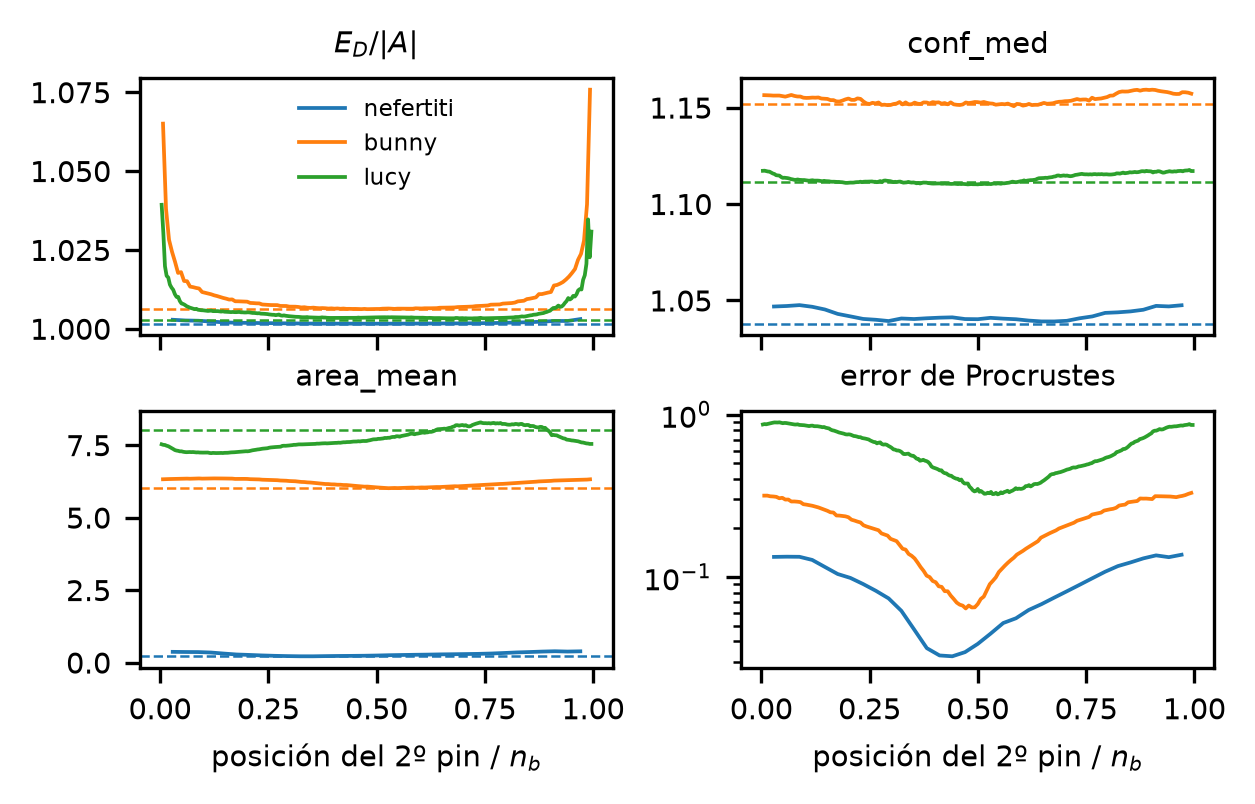
\includegraphics[width=\linewidth]{p3_pins.png}
\caption{Primer pin en la posición 0 y el segundo en todo el borde; segmentadas: pins automáticos.}
\end{subfigure}\hfill
\begin{subfigure}[b]{0.4\textwidth}\centering
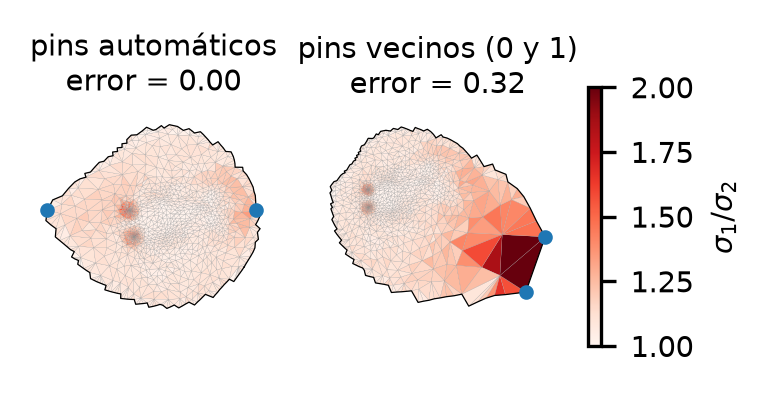
\includegraphics[width=\linewidth]{p3_pins_bunny.png}
\caption{Bunny: dominio $(u,v)$ alineado por Procrustes, coloreado por $\sigma_1/\sigma_2$.}
\end{subfigure}
\caption{Dependencia de LSCM respecto de los pins.}
\label{fig:pins}
\end{figure}

\preg{3.3} La Fig.~\ref{fig:pins}a muestra las tres medidas y el error de Procrustes en función de la posición del segundo pin. El error es la distancia relativa al resultado con pins automáticos después de alinear con la mejor semejanza (\code{comun.procrustes}, SVD sin reflexiones; validada: los mismos pins dan $10^{-16}$ y los pins intercambiados $10^{-12}$). Nunca es cero: mínimo 3, 6 y 32\,\% (Nefertiti, Bunny, Lucy) con pins opuestos, y 13, 32 y 87\,\% con pins vecinos. El resultado cambia más allá de una semejanza: en el caso discreto ningún mapa es exactamente conforme, y el mínimo restringido depende de qué vértices se fijan ($Qx\ne0$ solo en los pins, que actúan como fuerzas puntuales y deforman el mapa cerca de ellos). Con pins vecinos el efecto es fuerte: $E_D/|A|$ sube de 1.006 a 1.076 en Bunny y los triángulos cerca de los pins se agrandan y distorsionan (Fig.~\ref{fig:pins}b); \code{conf\_med} casi no cambia (es una mediana) y \code{area\_mean} varía hasta en 1 en Lucy. Recomendamos pins lejanos, aproximadamente opuestos en el borde, como hace \code{choose\_pins}: ahí las curvas son planas y el resultado es estable. Mejor aún es una formulación sin pins, como la parametrización conforme espectral de Mullen et al., que obtiene el mapa de un vector propio de $Q$.

\seccion{Parte 4. Análisis de las medidas de distorsión}
\preg{4.1} \code{jacobians} obtiene las coordenadas de cada triángulo en un sistema local isométrico ($q_0=0$, $q_1=(|p_1-p_0|,0)$, $q_2$ con $y_2>0$), forma $Q_m=[q_1-q_0\,|\,q_2-q_0]$ y $U_m=[u_1-u_0\,|\,u_2-u_0]$ y calcula $J=U_mQ_m^{-1}$ (ec.~10) para todas las caras a la vez. \code{face\_distortion} toma los valores singulares de $J$ y devuelve $\sigma_1/\sigma_2$ ($\infty$ si $\sigma_2\approx0$), $\log_2(\sigma_1\sigma_2)$ y $\det J$. Se trabaja en un sistema 2D porque el mapa afín va del \emph{plano del triángulo} a $\mathbb{R}^2$: con coordenadas 3D la matriz de aristas sería de $3\times2$, no invertible, y $J$ quedaría indefinido en la dirección normal. Como el sistema es isométrico, los $\sigma_i$ miden estiramiento real. Si se usa otro sistema isométrico $q'=Rq$ ($R$ ortogonal), entonces $Q_m'=RQ_m$ y $J'=U_mQ_m^{-1}R^T=JR^T$; luego $J'J'^T=JJ^T$ (mismos $\sigma_i$) y $\det J'=\det J\det R$, que conserva el signo si $R$ es una rotación y lo invierte si es una reflexión. El código fija $y_2>0$ (sistema orientado según el orden de los vértices de la cara), así que el signo es consistente. Experimento en Bunny con LSCM: rotar al azar el sistema de cada cara cambia $J$ hasta en 3.26, pero los $\sigma_i$ cambian menos de $10^{-15}$ y el signo de $\det J$ se mantiene en el 100\,\% de las caras (0\,\% con reflexión). Además $\det J=\det U_m/\det Q_m=A^{uv}_{\pm}/A^{3D}$: $|\det J|=\sigma_1\sigma_2$ es el cociente de áreas y su signo dice si se conserva la orientación (verificado con error $3\cdot10^{-16}$). \code{distortion\_report} reescala $(u,v)$ para que la media de $\log_2|\det J|$ sea 0, usa mediana y percentil 95 (robustos a unas pocas caras extremas) y llama degenerada a una cara con $|\det J|<10^{-12}\cdot$\,mediana.

\begin{table}[h]
\centering\small
\caption{Predicción (antes de calcular) / valor de \code{distortion\_report} en la malla plana de prueba (392 caras).}
\label{tab:p4}
\begin{tabular}{llccc}
\toprule
mapa & $J$ & \code{conf\_med} & \code{area\_mean} & \code{flips} \\
\midrule
(a) rotación 30 grados y escala 2 & $2R$ & 1 / 1.000 & 0 / 0.000 & 0 / 0 \\
(b) $(x,y)\to(3x,y)$ & $\operatorname{diag}(3,1)$ & 3 / 3.000 & 0 / 0.000 & 0 / 0 \\
(c) $(x,y)\to(x+0.5y,y)$ & $\begin{psmallmatrix}1&0.5\\0&1\end{psmallmatrix}$ & $\left(\frac{0.5+\sqrt{4.25}}{2}\right)^2=1.640$ / 1.640 & 0 / 0.000 & 0 / 0 \\
(d) $(x,y)\to(-x,y)$ & $\operatorname{diag}(-1,1)$ & 1 / 1.000 & 0 / 0.000 & 392 / \textbf{0} \\
(e) $z\to z^2$, $z=(x+1)+iy$ & $f'(z)=2z$ & 1 / \textbf{1.034} & 0.447 / 0.447 & 0 / 0 \\
\bottomrule
\end{tabular}
\end{table}

\preg{4.2} La Tabla~\ref{tab:p4} compara las predicciones (en el código, \code{p4\_distorsion.predicciones}) con lo medido, y la Fig.~\ref{fig:p4} muestra el tablero: rectángulos 1:3 en (b), paralelogramos en (c) y cuadrados curvos de tamaño variable en (e). Coinciden salvo en dos casos, y ambos se explican por el método. En (d) la reflexión invierte todas las caras, pero el reporte cuenta flips respecto de la orientación dominante ($\operatorname{sign}\sum\det J\,A$), así que una reflexión global no cuenta; en el tablero tampoco se nota, porque es simétrico. En (e) $z^2$ es conforme, pero su interpolación lineal en cada triángulo no lo es exactamente: \code{conf\_med} 1.034, con error del orden de $h|f''|/|f'|$. Además, en (a)--(c) \code{area\_mean} es 0 aunque el área total se multiplique por 4, 3 y 1, porque la normalización de escala solo mide variaciones relativas de área. En (e) el área local $4|z|^2$ varía 5 veces y \code{area\_mean} coincide con la integral continua (0.447).

\begin{figure}[t]
\centering
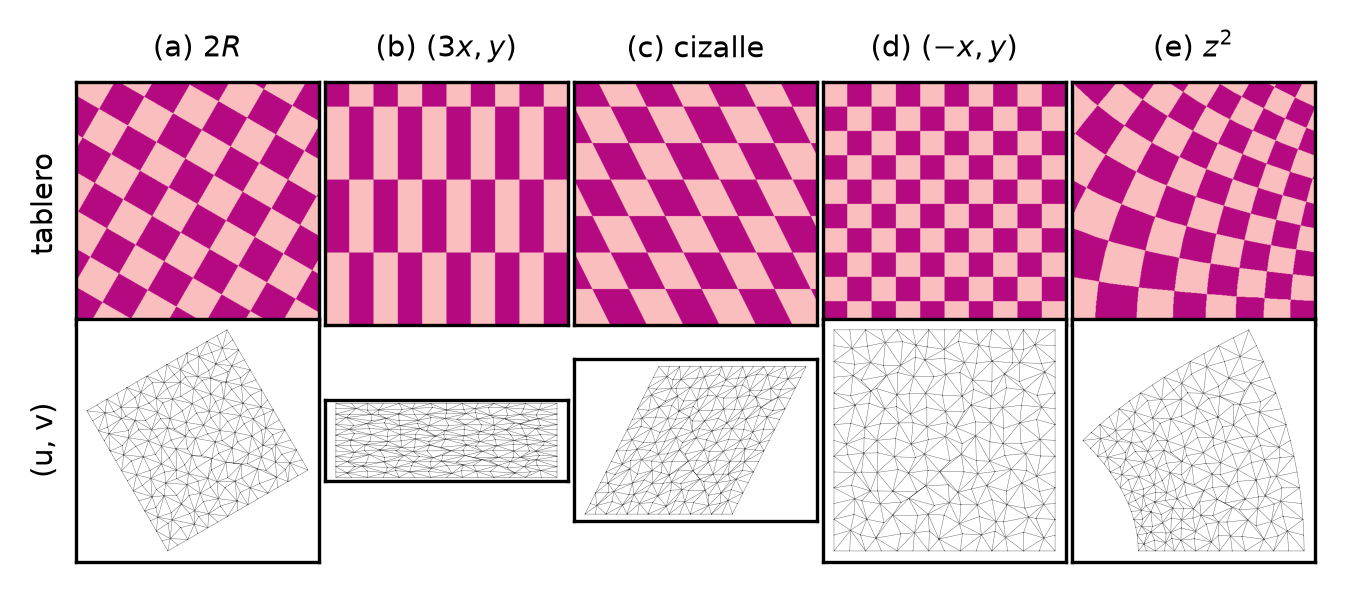
\includegraphics[width=0.64\textwidth]{p4_experimentos.png}
\caption{Experimentos controlados: arriba, tablero sobre la malla plana; abajo, dominio $(u,v)$.}
\label{fig:p4}
\end{figure}

\seccion{Parte 5. Análisis comparativo}
La Fig.~\ref{fig:tableros}a resume los cuatro métodos; el Anexo~\ref{anx:mosaicos} tiene, para cada malla, el tablero, el dominio $(u,v)$ y los mapas de distorsión conforme y de área.

\begin{figure}[t]
\centering
\begin{subfigure}[b]{0.57\textwidth}\centering
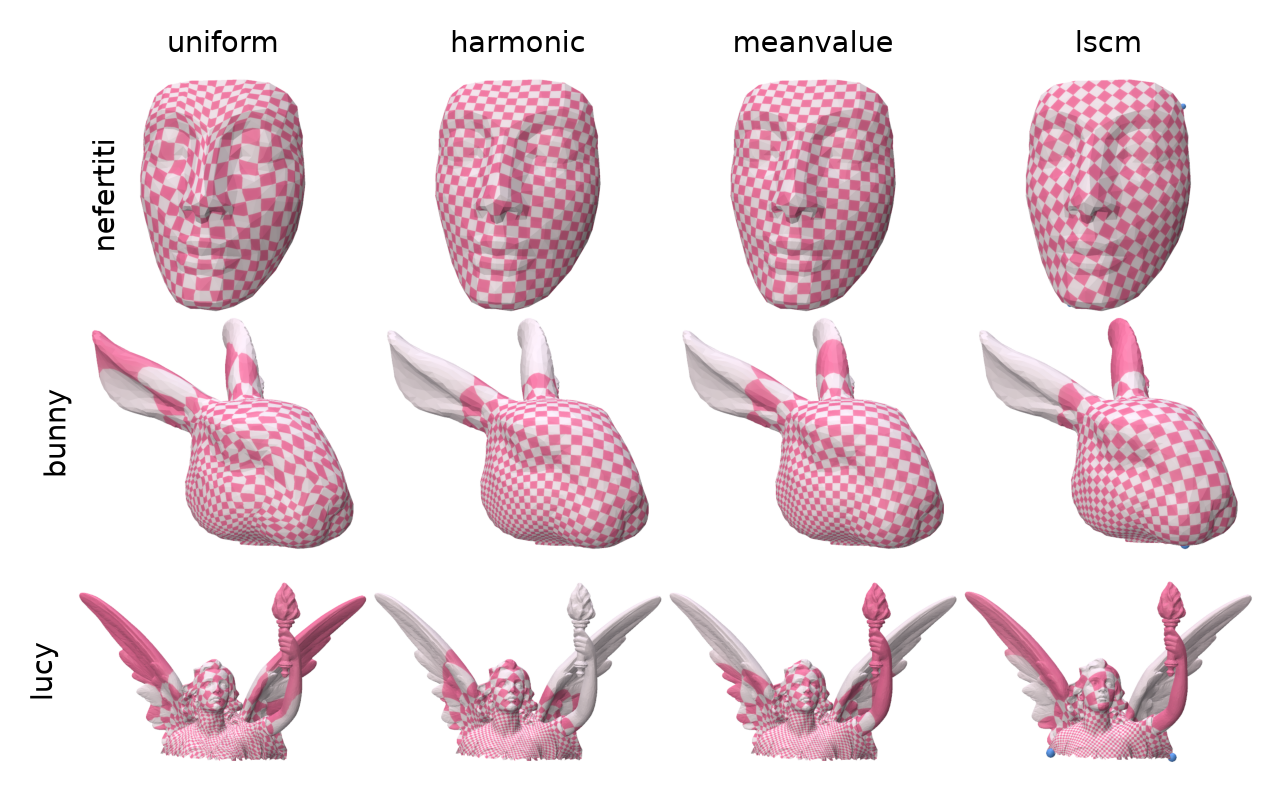
\includegraphics[width=\linewidth]{p5_tableros.png}
\caption{Tablero sobre la superficie (casilla 0.04, 0.02 y 0.015 en $(u,v)$ normalizado; puntos azules: pins de LSCM).}
\end{subfigure}\hfill
\begin{subfigure}[b]{0.4\textwidth}\centering
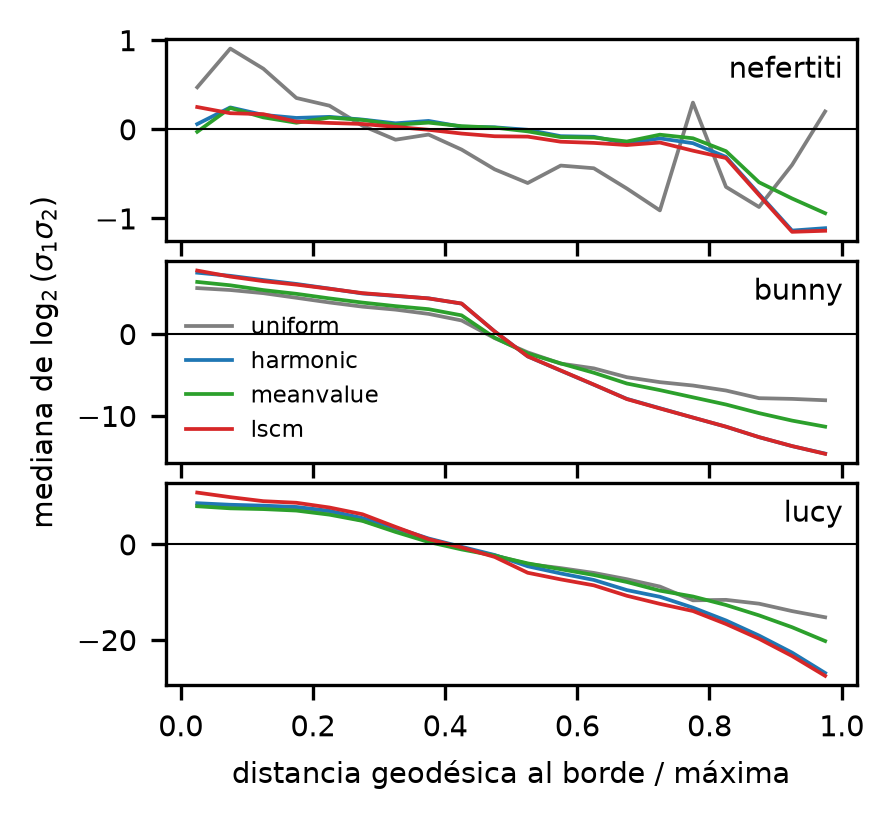
\includegraphics[width=\linewidth]{p5_area_vs_distancia.png}
\caption{Mediana de $\log_2(\sigma_1\sigma_2)$ (sin caras degeneradas) según la distancia al borde.}
\end{subfigure}
\caption{Los cuatro métodos en las tres mallas (borde fijo: círculo y \code{arc}).}
\label{fig:tableros}
\end{figure}

\begin{table}[h]
\centering\small
\caption{\code{conf\_med} y \code{area\_mean} (borde circular, \code{arc}); entre paréntesis, el lugar en cada malla.}
\label{tab:orden}
\begin{tabular}{lcccccc}
\toprule
& \multicolumn{2}{c}{Nefertiti} & \multicolumn{2}{c}{Bunny} & \multicolumn{2}{c}{Lucy} \\
\cmidrule(lr){2-3}\cmidrule(lr){4-5}\cmidrule(lr){6-7}
método & conforme & área & conforme & área & conforme & área \\
\midrule
uniform & 1.538 (4) & 0.580 (4) & 1.770 (4) & 4.092 (1) & 2.042 (4) & 6.815 (2) \\
harmonic & 1.144 (2) & 0.202 (2) & 1.191 (2) & 6.037 (4) & 1.262 (2) & 7.594 (3) \\
meanvalue & 1.165 (3) & 0.178 (1) & 1.268 (3) & 4.629 (2) & 1.402 (3) & 6.740 (1) \\
lscm & 1.038 (1) & 0.219 (3) & 1.152 (1) & 6.030 (3) & 1.111 (1) & 8.028 (4) \\
\bottomrule
\end{tabular}
\end{table}

\preg{5.1} En distorsión conforme el orden es igual en las tres mallas: LSCM $<$ armónico $<$ valor medio $<$ uniforme (Tabla~\ref{tab:orden}). En área cambia: valor medio gana en Nefertiti y Lucy, uniforme en Bunny, y LSCM queda tercero o último. Ningún método gana en ambas. Un mapa que conserve ángulos y áreas tiene $\sigma_1=\sigma_2=1$, o sea, es una isometría; por el Teorema Egregium conserva la curvatura de Gauss, y como el plano tiene $K=0$, solo una superficie desarrollable se puede aplanar sin distorsión. En una superficie curva hay que elegir: un mapa conforme pone toda la distorsión en el factor de escala (como $z^2$ en 4.2), y uno que conserve área tiene que deformar ángulos.

\preg{5.2} En un mapa conforme el logaritmo del factor de escala, $\varphi=\log\sigma$, cumple $\Delta_S\varphi=K$, así que la curvatura se paga en escala. Una protuberancia es como un tubo de perímetro $c$ y largo $\ell$ pegado al cuerpo, y un tubo solo se aplana conformemente como un anillo de radios $r$ y $R=re^{2\pi\ell/c}$. El extremo se encoge en un factor $e^{-2\pi\ell/c}$ en longitud y $e^{-4\pi\ell/c}$ en área, es decir, exponencialmente en $\ell/c$ (con $\ell\approx c$, $e^{-4\pi}\approx2^{-18}$). Los mapas armónicos de borde fijo se comportan igual, y el borde libre de LSCM no ayuda: el borde está en la base de Bunny y de Lucy, lejos de las protuberancias, y la oreja se sigue aplanando ``a través de'' su base. La Fig.~\ref{fig:tableros}b lo confirma: la mediana de $\log_2(\sigma_1\sigma_2)$ cae casi linealmente con la distancia geodésica al borde, hasta $-15$ en las orejas de Bunny y $-27$ en las alas y la antorcha de Lucy. Los mínimos llegan a $-37$, y las caras bajo $2^{-40}$ son los \code{degen} de Lucy (también con el círculo). Los métodos más conformes (armónico, LSCM) son los que más comprimen. La pregunta 4.5 citada no existe en el enunciado; usando lo observado en la Parte 4 (un mapa conforme puede cambiar el área arbitrariamente, como $z^2$), proponemos: (i) cortar costuras desde la punta de cada protuberancia hasta el borde, para que pase a ser parte del borde libre y LSCM la desenrolle (un tubo cortado a lo largo es desarrollable); (ii) un atlas de varias cartas; o (iii) singularidades cónicas en las puntas, o una energía que también penalice la distorsión de área (p.\,ej.\ ARAP).

\preg{5.3} Elegiríamos LSCM (borde libre). Es el más conforme en Nefertiti (\code{conf\_med} 1.038, \code{conf\_p95} 1.201, $E_D/|A|=1.0016$), su distorsión de área es baja (0.219, similar a 0.178--0.202 de valor medio y armónico) y no tiene flips. En una foto importa sobre todo conservar ángulos (las proporciones de ojos y boca), y un borde fijo agrega distorsión: el círculo en la frente y el mentón (\code{conf\_p95} 1.394 con armónico), el cuadrado mucho más (\code{conf\_p95} 2.472; en la Fig.~\ref{fig:foto}e la gorra de la foto invade la frente). La Fig.~\ref{fig:foto} muestra la foto aplicada con los tres. Si se necesitara un borde fijo, usaríamos valor medio o armónico con círculo y espaciado \code{arc}.

\begin{table}[h]
\centering\small
\caption{Tiempos en Lucy (mediana de 5 repeticiones, en segundos).}
\label{tab:tiempos}
\begin{tabular}{lrrrrrr}
\toprule
método & pesos & otras etapas & factorización LU & sustitución & total & incógnitas \\
\midrule
uniform & 0.063 & 0.003 & 0.042 & 0.004 & 0.114 & 13\,894 \\
harmonic & 0.015 & 0.003 & 0.043 & 0.004 & 0.064 & 13\,894 \\
meanvalue & 0.022 & 0.003 & 0.042 & 0.004 & 0.073 & 13\,894 \\
lscm & 0.014 & 0.005 & 0.101 & 0.004 & 0.121 & 28\,308 \\
\bottomrule
\end{tabular}

\end{table}

\preg{5.4} La Tabla~\ref{tab:tiempos} separa las etapas de \code{parameterize} en Lucy (14\,156 vértices): ``otras etapas'' son el Laplaciano, el borde o la matriz $Q$, y la extracción de submatrices. El total es del orden de 0.1\,s. En armónico, valor medio y LSCM domina la factorización LU dispersa (SuperLU): 0.04\,s con 13\,894 incógnitas en los de borde fijo y 0.10\,s en LSCM, que tiene el doble de incógnitas y acopla $u$ con $v$ (más relleno). En uniforme domina construir los pesos (unos 0.06\,s), por el \code{np.unique} de \code{unique\_edges}; los pesos vectorizados cotangentes y de valor medio cuestan unos 0.02\,s. Las sustituciones y el resto cuestan milisegundos, y medir la distorsión (0.05\,s) cuesta casi lo mismo que parametrizar.

\begin{figure}[tb]
\centering
\begin{subfigure}{0.19\textwidth}\centering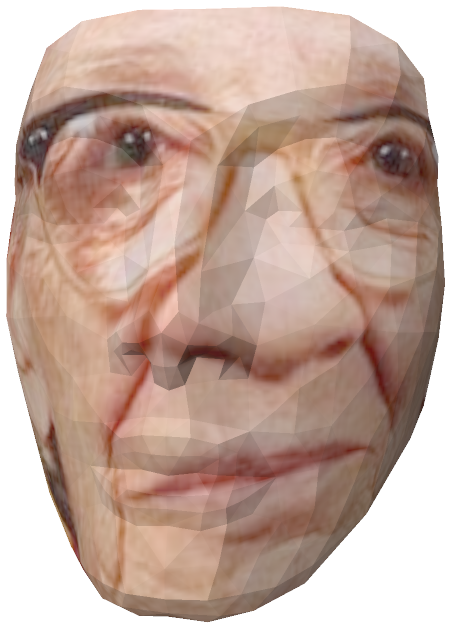
\includegraphics[height=3.0cm]{b2_lscm_libre_frente.png}\caption{LSCM}\end{subfigure}\hfill
\begin{subfigure}{0.19\textwidth}\centering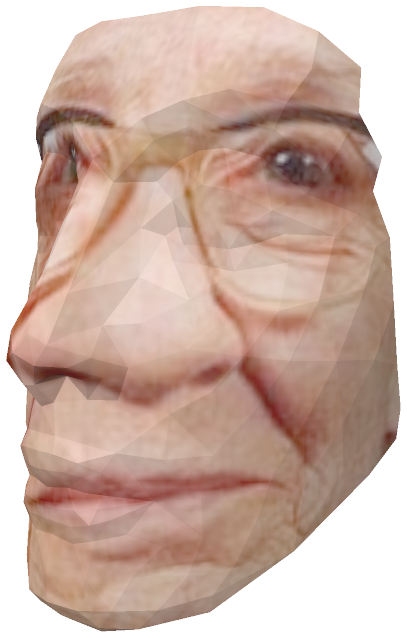
\includegraphics[height=3.0cm]{b2_lscm_libre_lado.png}\caption{LSCM}\end{subfigure}\hfill
\begin{subfigure}{0.2\textwidth}\centering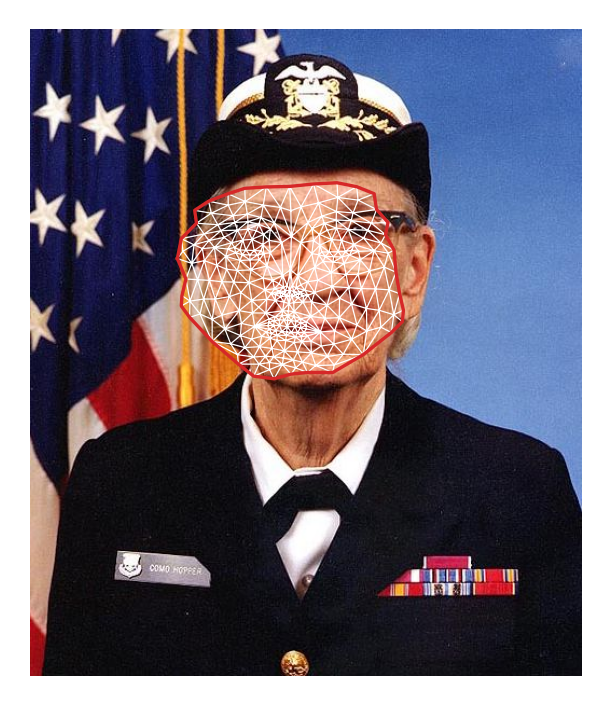
\includegraphics[height=3.0cm]{b2_lscm_libre_uv.png}\caption{foto y $(u,v)$}\end{subfigure}\hfill
\begin{subfigure}{0.19\textwidth}\centering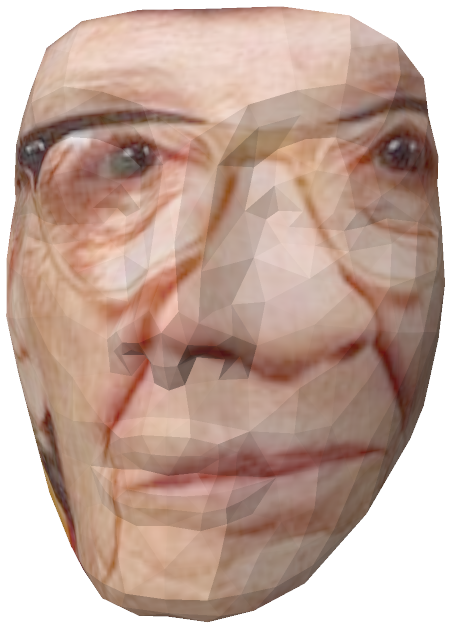
\includegraphics[height=3.0cm]{b2_harmonic_circle_frente.png}\caption{armónico + círculo}\end{subfigure}\hfill
\begin{subfigure}{0.19\textwidth}\centering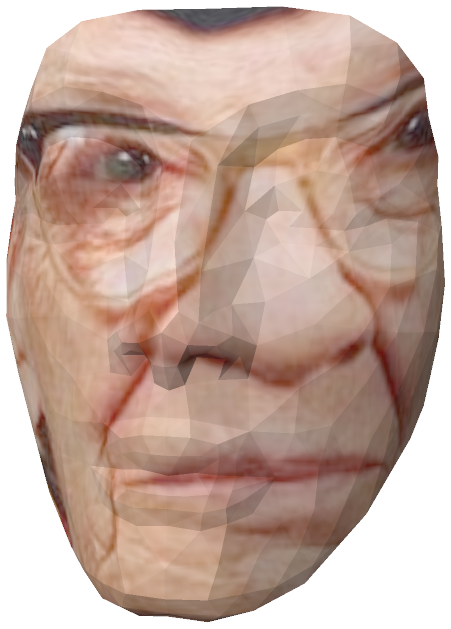
\includegraphics[height=3.0cm]{b2_meanvalue_square_frente.png}\caption{v.\ medio + cuadrado}\end{subfigure}
\caption{Bonus B2: fotografía como textura de Nefertiti.}
\label{fig:foto}
\end{figure}

\seccion{Bonus}
\preg{B1} \code{bulged\_square\_points} (en \code{boundary.py}, forma \code{"bulged\_square"}) desplaza cada punto del cuadrado hacia afuera en $4b\,s(1-s)$, donde $s$ es su posición en el lado y $b=0.05$. Cada lado queda como un arco de parábola y la curva es estrictamente convexa, así que tres vértices del borde nunca son colineales y vale el teorema completo. Resultado (Anexo~\ref{anx:extra}): \code{degen}~=~0 en Nefertiti y en Bunny (antes 4) con los tres pesos, sin flips, y \code{conf\_med} incluso mejora respecto del cuadrado (1.409 $\to$ 1.378 con valor medio en Bunny). En Lucy desaparecen las 23 caras degeneradas del borde. Las que quedan (179/1\,419/983) son las mismas que con el círculo (184/1\,418/978): están a 44 anillos o más del borde, en las puntas de alas y antorcha, y se deben a la compresión de 5.2. Ninguna curva de borde las evita.

\preg{B2} \code{b2\_foto.py} aplica una fotografía real (Grace Hopper, incluida en Matplotlib) como textura de Nefertiti con Polyscope (\code{add\_color\_quantity(..., defined\_on="texture")}). Para que la cara de la foto quede sobre la de la malla, se marcan los ojos y la boca en ambas y se calcula con Procrustes la semejanza que lleva unos a otros. Aplicarla a todo $(u,v)$ no agrega distorsión (Fig.~\ref{fig:foto}).

% ---------------------------------------------------------------------------
\clearpage
\appendix
\renewcommand{\thesection}{\Alph{section}}
\section{Tablas \code{--batch} completas}\label{anx:tablas}
\begin{table}[h]
\centering\scriptsize
\caption{Nefertiti (299 vértices, 562 caras, 34 en el borde).}
\begin{tabular}{lllrrrrrrrr}
\toprule
método & borde & espaciado & neg\_w & conf\_med & conf\_p95 & area\_mean & flips & degen & $E_D/|A|$ & tiempo [s] \\
\midrule
uniform & circle & arc & 0 & 1.538 & 2.700 & 0.580 & 0 & 0 & 1.2174 & 0.004 \\
uniform & circle & uniform & 0 & 1.581 & 2.929 & 0.594 & 0 & 0 & 1.2583 & 0.002 \\
uniform & square & arc & 0 & 1.670 & 3.444 & 0.587 & 0 & 0 & 1.3402 & 0.002 \\
uniform & square & uniform & 0 & 1.669 & 3.709 & 0.580 & 0 & 0 & 1.4101 & 0.002 \\
uniform & star & arc & 0 & 1.746 & 7.372 & 0.702 & 13 & 0 & 1.8106 & 0.002 \\
uniform & star & uniform & 0 & 1.790 & 5.960 & 0.671 & 15 & 0 & 1.8063 & 0.002 \\
\midrule
harmonic & circle & arc & 86 & 1.144 & 1.394 & 0.202 & 0 & 0 & 1.0217 & 0.002 \\
harmonic & circle & uniform & 86 & 1.205 & 1.619 & 0.285 & 0 & 0 & 1.0549 & 0.002 \\
harmonic & square & arc & 86 & 1.360 & 2.288 & 0.224 & 0 & 0 & 1.1216 & 0.002 \\
harmonic & square & uniform & 86 & 1.373 & 2.755 & 0.321 & 0 & 0 & 1.1807 & 0.002 \\
harmonic & star & arc & 86 & 1.470 & 6.111 & 0.468 & 12 & 0 & 1.5087 & 0.002 \\
harmonic & star & uniform & 86 & 1.483 & 5.470 & 0.465 & 13 & 0 & 1.5170 & 0.002 \\
\midrule
meanvalue & circle & arc & 0 & 1.165 & 1.441 & 0.178 & 0 & 0 & 1.0234 & 0.002 \\
meanvalue & circle & uniform & 0 & 1.237 & 1.634 & 0.253 & 0 & 0 & 1.0575 & 0.002 \\
meanvalue & square & arc & 0 & 1.354 & 2.472 & 0.227 & 0 & 0 & 1.1258 & 0.002 \\
meanvalue & square & uniform & 0 & 1.381 & 3.035 & 0.307 & 0 & 0 & 1.1861 & 0.002 \\
meanvalue & star & arc & 0 & 1.431 & 6.727 & 0.630 & 14 & 0 & 1.5194 & 0.002 \\
meanvalue & star & uniform & 0 & 1.483 & 6.045 & 0.497 & 16 & 0 & 1.5270 & 0.002 \\
\midrule
lscm & - & - & 0 & 1.038 & 1.201 & 0.219 & 0 & 0 & 1.0016 & 0.004 \\
\bottomrule
\end{tabular}

\end{table}
\begin{table}[h]
\centering\scriptsize
\caption{Bunny (1\,573 vértices, 3\,000 caras, 144 en el borde).}
\begin{tabular}{lllrrrrrrrr}
\toprule
método & borde & espaciado & neg\_w & conf\_med & conf\_p95 & area\_mean & flips & degen & $E_D/|A|$ & tiempo [s] \\
\midrule
uniform & circle & arc & 0 & 1.770 & 3.446 & 4.092 & 0 & 0 & 1.1678 & 0.011 \\
uniform & circle & uniform & 0 & 1.785 & 3.469 & 4.104 & 0 & 0 & 1.1693 & 0.010 \\
uniform & square & arc & 0 & 1.885 & 3.683 & 4.075 & 0 & 4 & 1.2727 & 0.010 \\
uniform & square & uniform & 0 & 1.885 & 3.773 & 4.085 & 0 & 4 & 1.2684 & 0.010 \\
uniform & star & arc & 0 & 1.951 & 6.216 & 4.029 & 41 & 4 & 1.7456 & 0.010 \\
uniform & star & uniform & 0 & 1.960 & 6.050 & 4.056 & 48 & 4 & 1.7392 & 0.011 \\
\midrule
harmonic & circle & arc & 922 & 1.191 & 1.560 & 6.037 & 0 & 0 & 1.0270 & 0.006 \\
harmonic & circle & uniform & 922 & 1.198 & 1.594 & 6.050 & 0 & 0 & 1.0293 & 0.006 \\
harmonic & square & arc & 922 & 1.274 & 2.007 & 6.023 & 0 & 4 & 1.1213 & 0.006 \\
harmonic & square & uniform & 922 & 1.289 & 1.978 & 6.036 & 0 & 4 & 1.1189 & 0.006 \\
harmonic & star & arc & 922 & 1.311 & 5.295 & 5.984 & 28 & 4 & 1.5469 & 0.007 \\
harmonic & star & uniform & 922 & 1.323 & 5.331 & 5.997 & 42 & 4 & 1.5496 & 0.006 \\
\midrule
meanvalue & circle & arc & 0 & 1.268 & 2.105 & 4.629 & 0 & 0 & 1.0333 & 0.007 \\
meanvalue & circle & uniform & 0 & 1.278 & 2.134 & 4.641 & 0 & 0 & 1.0354 & 0.007 \\
meanvalue & square & arc & 0 & 1.409 & 2.368 & 4.616 & 0 & 4 & 1.1283 & 0.007 \\
meanvalue & square & uniform & 0 & 1.415 & 2.406 & 4.623 & 0 & 4 & 1.1258 & 0.011 \\
meanvalue & star & arc & 0 & 1.439 & 5.114 & 4.567 & 27 & 4 & 1.5632 & 0.011 \\
meanvalue & star & uniform & 0 & 1.440 & 5.111 & 4.595 & 39 & 4 & 1.5700 & 0.008 \\
\midrule
lscm & - & - & 0 & 1.152 & 1.460 & 6.030 & 0 & 0 & 1.0064 & 0.012 \\
\bottomrule
\end{tabular}

\end{table}
\begin{table}[h]
\centering\scriptsize
\caption{Lucy (14\,156 vértices, 28\,048 caras, 262 en el borde). Los \code{degen} con el círculo son caras de las protuberancias comprimidas bajo $2^{-40}$ (pregunta 5.2).}
\begin{tabular}{lllrrrrrrrr}
\toprule
método & borde & espaciado & neg\_w & conf\_med & conf\_p95 & area\_mean & flips & degen & $E_D/|A|$ & tiempo [s] \\
\midrule
uniform & circle & arc & 0 & 2.042 & 4.888 & 6.815 & 0 & 184 & 1.4276 & 0.107 \\
uniform & circle & uniform & 0 & 2.076 & 5.038 & 6.862 & 0 & 145 & 1.4601 & 0.163 \\
uniform & square & arc & 0 & 2.110 & 5.244 & 6.787 & 0 & 202 & 1.5243 & 0.162 \\
uniform & square & uniform & 0 & 2.052 & 5.075 & 6.838 & 0 & 162 & 1.5483 & 0.165 \\
uniform & star & arc & 0 & 2.763 & 9.134 & 6.753 & 273 & 176 & 2.0537 & 0.184 \\
uniform & star & uniform & 0 & 2.801 & 9.705 & 6.757 & 327 & 170 & 2.1590 & 0.164 \\
\midrule
harmonic & circle & arc & 11192 & 1.262 & 1.690 & 7.594 & 1 & 1418 & 1.0615 & 0.094 \\
harmonic & circle & uniform & 11192 & 1.339 & 1.774 & 7.632 & 1 & 1394 & 1.0827 & 0.091 \\
harmonic & square & arc & 11192 & 1.394 & 2.113 & 7.560 & 1 & 1442 & 1.1359 & 0.094 \\
harmonic & square & uniform & 11192 & 1.313 & 1.919 & 7.604 & 1 & 1420 & 1.1534 & 0.093 \\
harmonic & star & arc & 11192 & 2.067 & 4.448 & 7.523 & 238 & 1437 & 1.5519 & 0.091 \\
harmonic & star & uniform & 11192 & 2.075 & 4.537 & 7.521 & 237 & 1434 & 1.6090 & 0.090 \\
\midrule
meanvalue & circle & arc & 0 & 1.402 & 2.856 & 6.740 & 0 & 978 & 1.0733 & 0.103 \\
meanvalue & circle & uniform & 0 & 1.466 & 2.959 & 6.803 & 0 & 927 & 1.0949 & 0.101 \\
meanvalue & square & arc & 0 & 1.403 & 2.835 & 6.701 & 0 & 1008 & 1.1505 & 0.102 \\
meanvalue & square & uniform & 0 & 1.376 & 2.698 & 6.772 & 0 & 957 & 1.1680 & 0.102 \\
meanvalue & star & arc & 0 & 2.020 & 5.683 & 6.665 & 159 & 992 & 1.5781 & 0.102 \\
meanvalue & star & uniform & 0 & 1.845 & 5.405 & 6.672 & 197 & 980 & 1.6363 & 0.102 \\
\midrule
lscm & - & - & 0 & 1.111 & 1.360 & 8.028 & 1 & 1232 & 1.0028 & 0.155 \\
\bottomrule
\end{tabular}

\end{table}

\clearpage
\section{Los cuatro métodos en cada malla}\label{anx:mosaicos}
Filas: tablero sobre la superficie, dominio $(u,v)$ con su borde en rojo, distorsión conforme $\sigma_1/\sigma_2$ (blanco = 1) y de área $\log_2(\sigma_1\sigma_2)$ (azul = comprimido, rojo = expandido). Los fijos usan círculo y espaciado \code{arc}. En Lucy, la llama de la antorcha aparece roja en el mapa conforme y blanca en el de área porque sus caras son degeneradas (el reporte les asigna $\sigma_1/\sigma_2=10^{12}$ y área 0).

\begin{figure}[h]
\centering
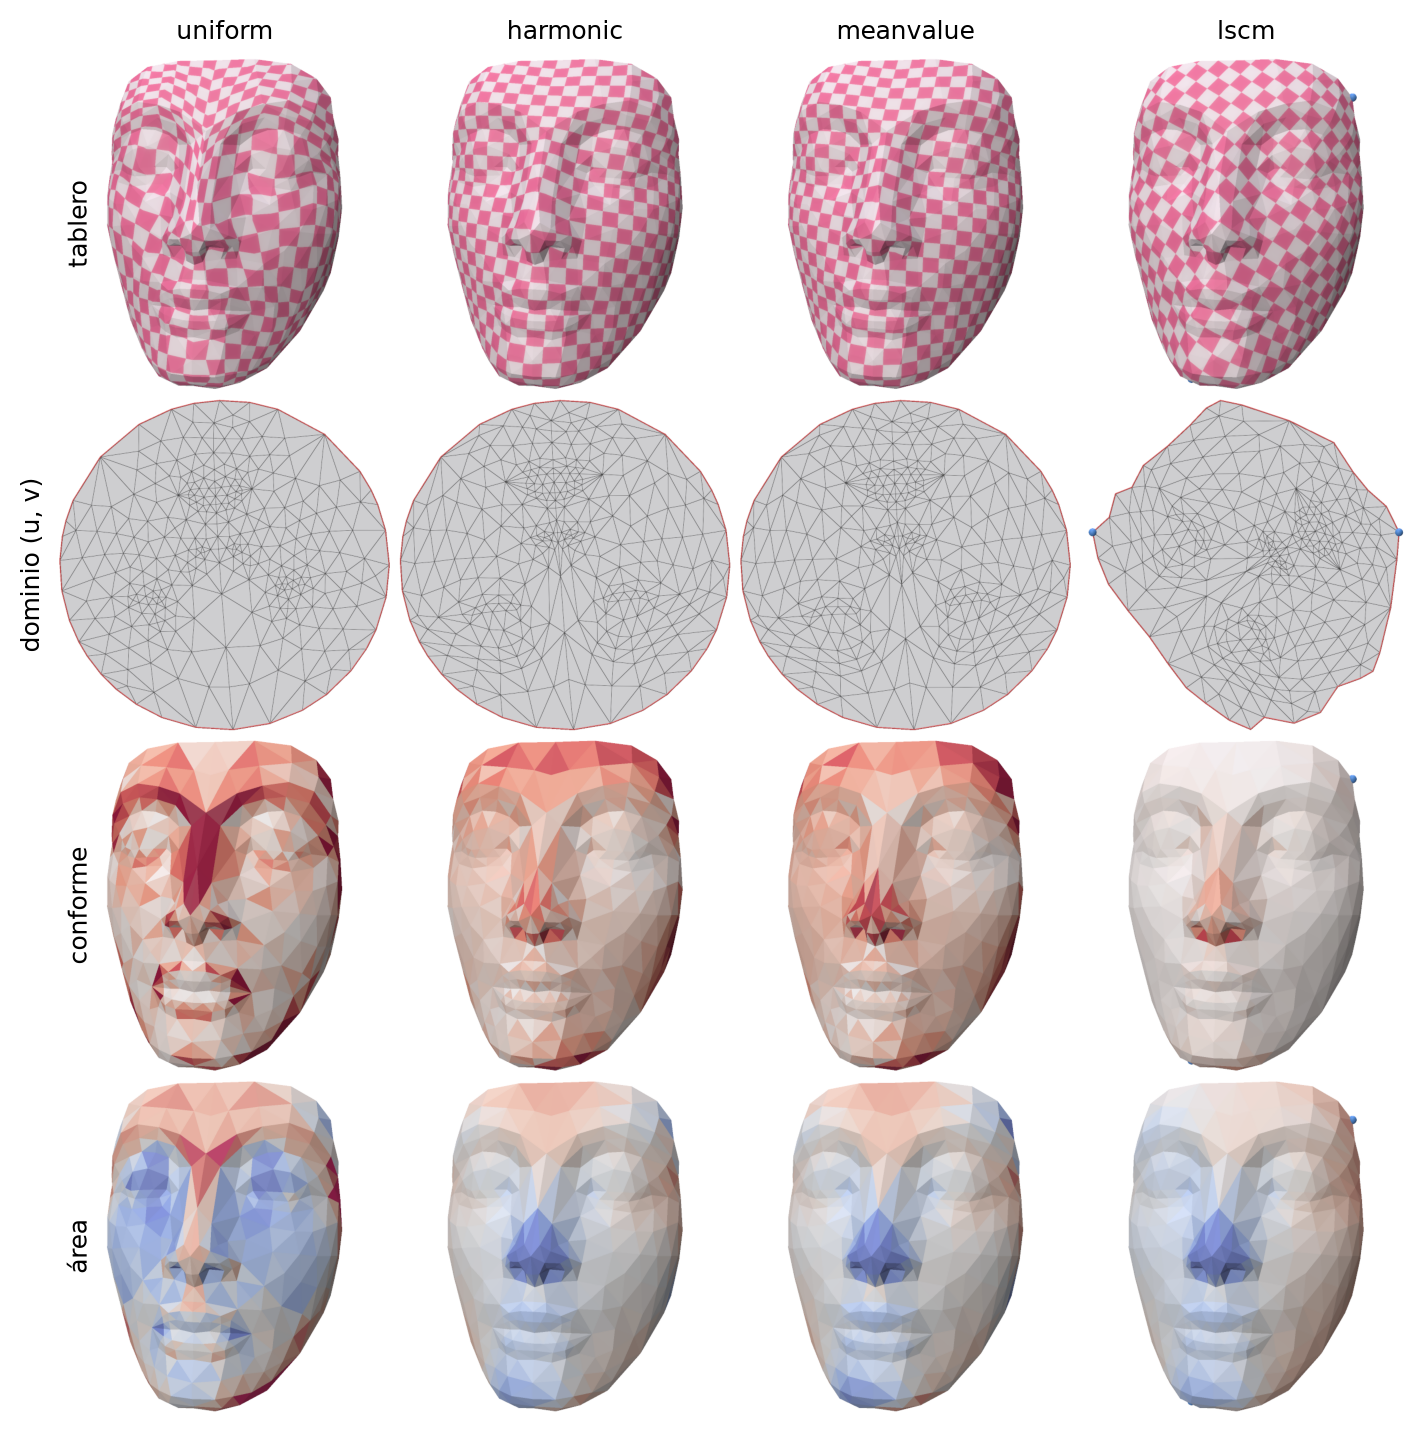
\includegraphics[width=0.78\textwidth]{p5_mosaico_nefertiti.png}
\caption{Nefertiti.}
\end{figure}
\begin{figure}[p]
\centering
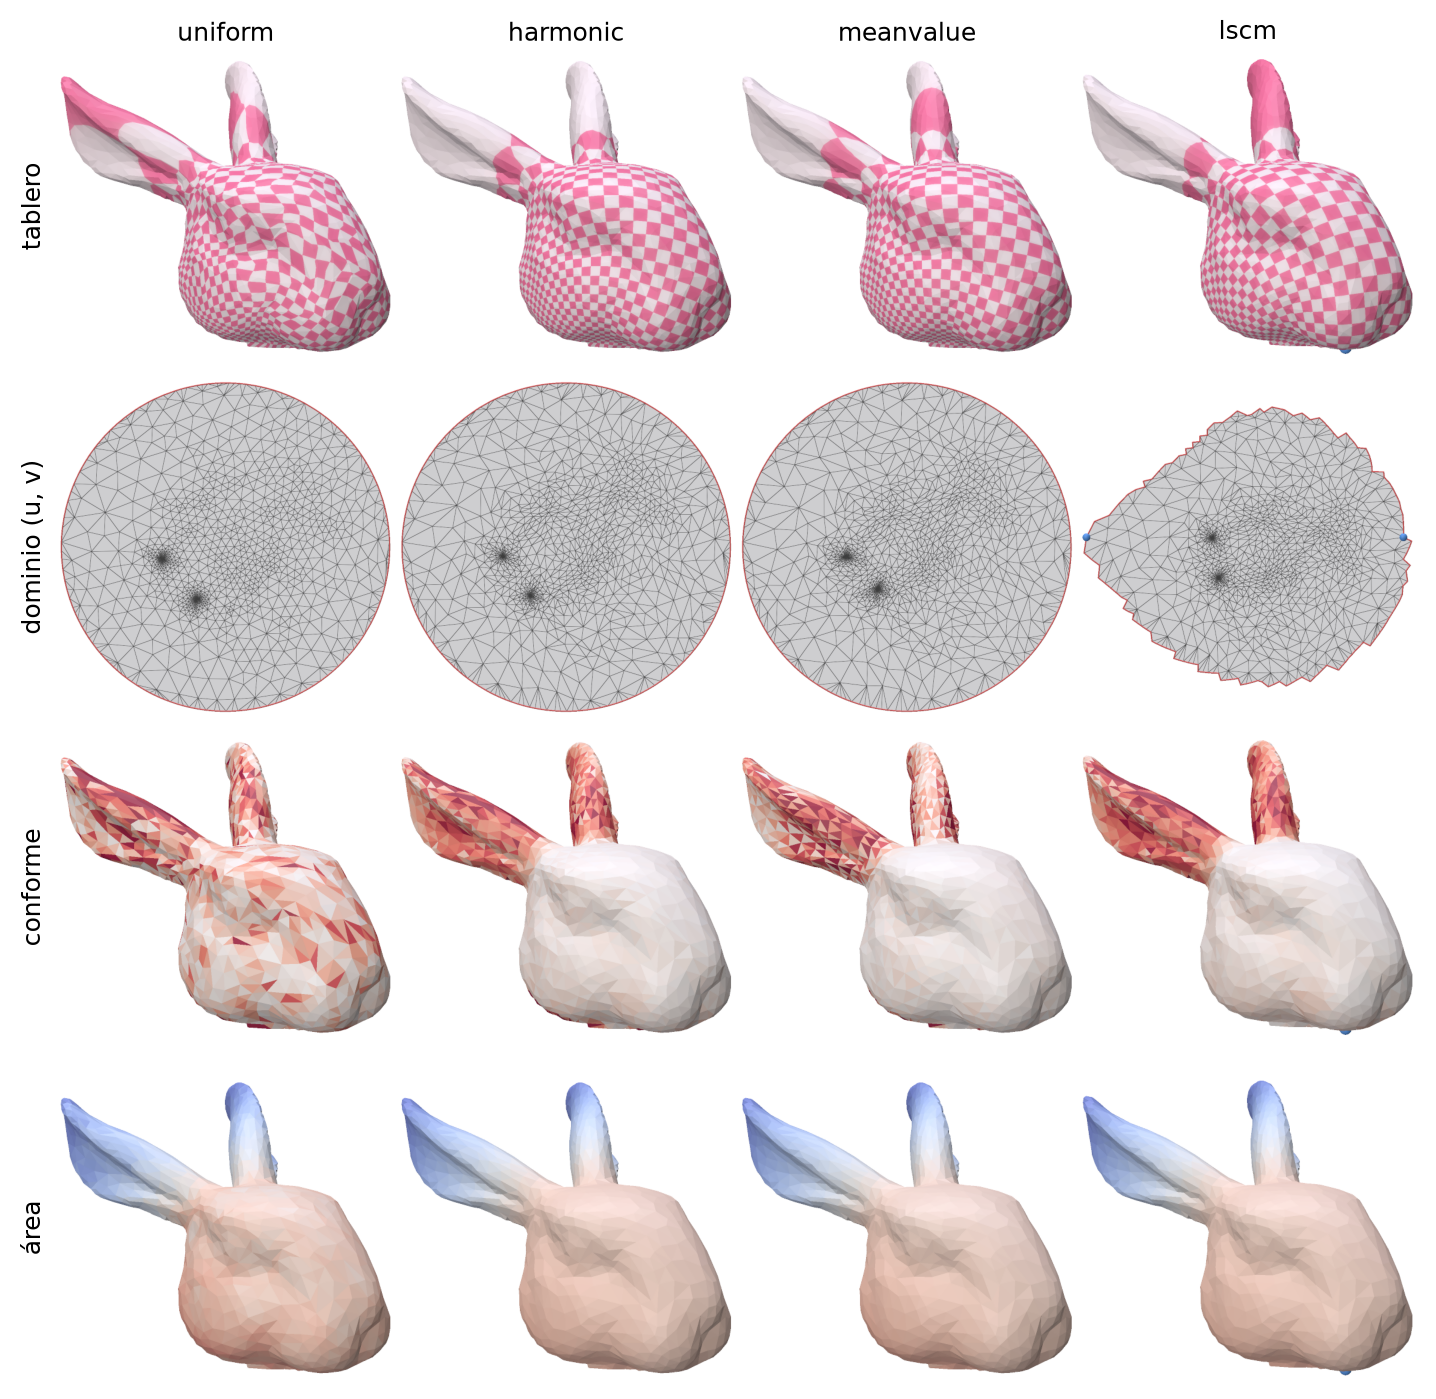
\includegraphics[width=0.84\textwidth]{p5_mosaico_bunny.png}
\caption{Bunny.}
\end{figure}
\begin{figure}[p]
\centering
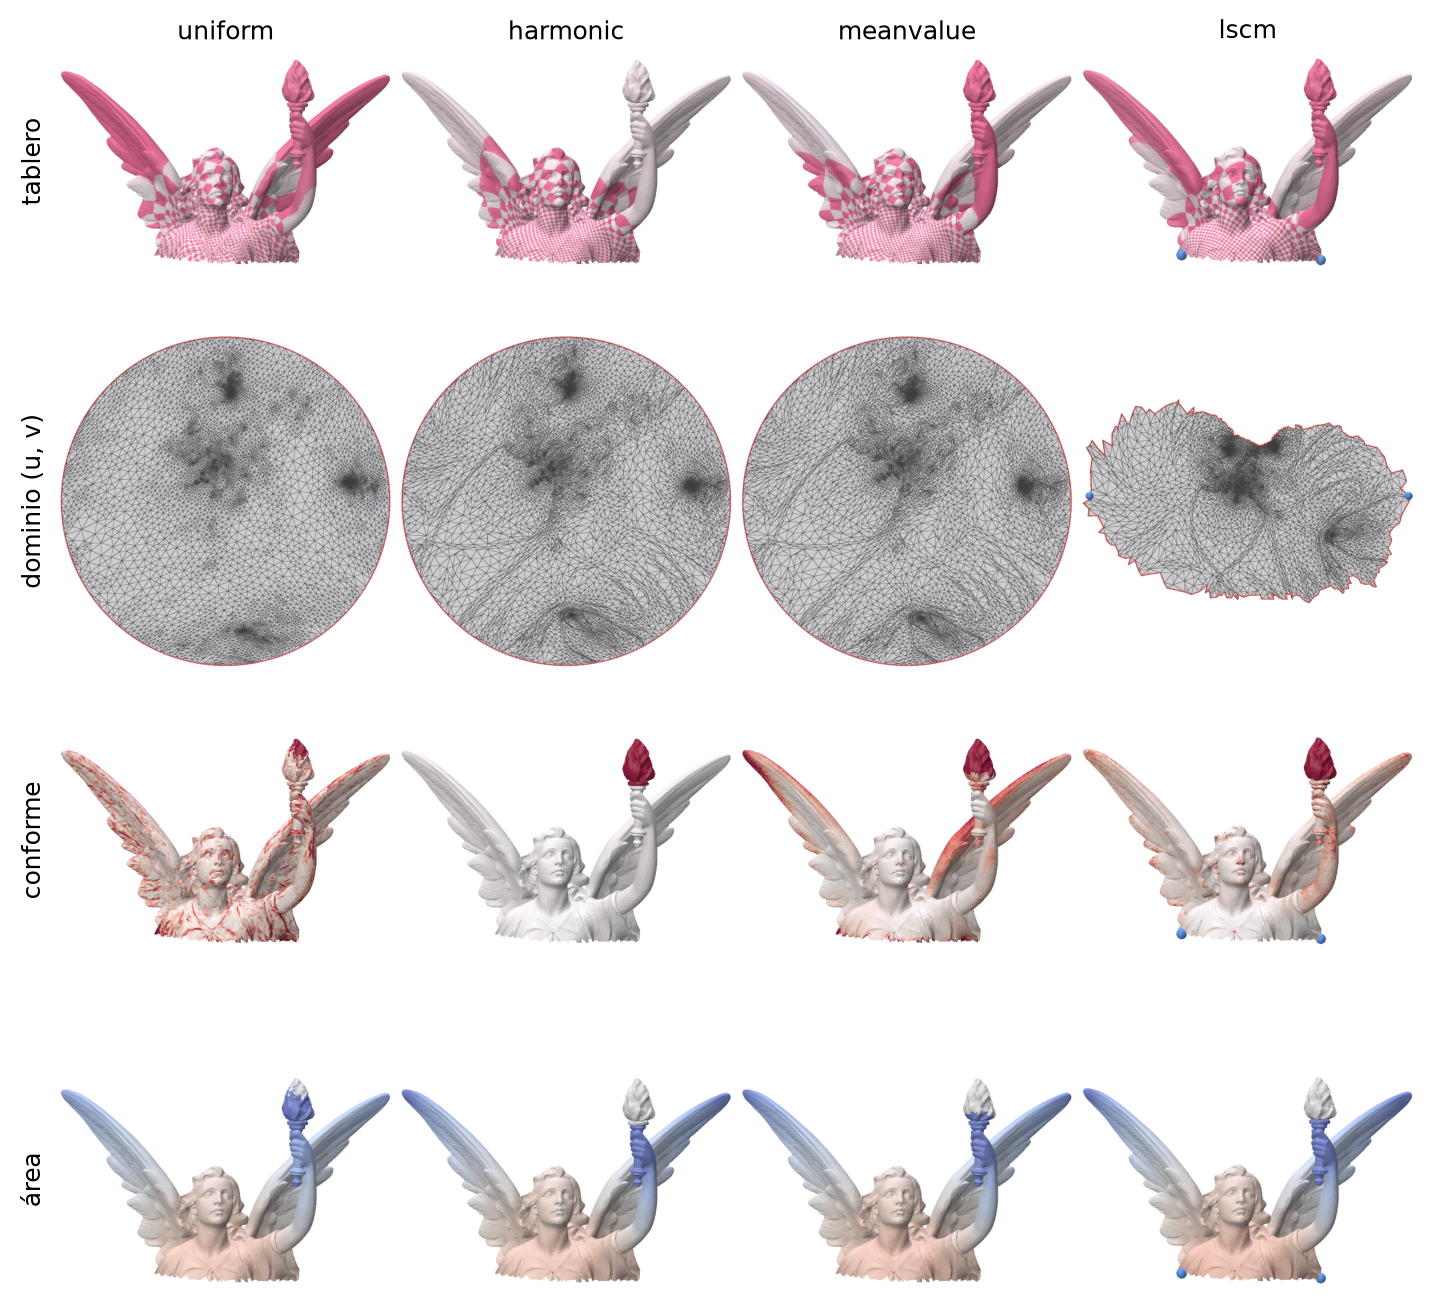
\includegraphics[width=0.84\textwidth]{p5_mosaico_lucy.png}
\caption{Lucy.}
\end{figure}

\clearpage
\section{Figuras y tablas adicionales}\label{anx:extra}
\begin{figure}[h]
\centering
\begin{subfigure}{0.2\textwidth}\centering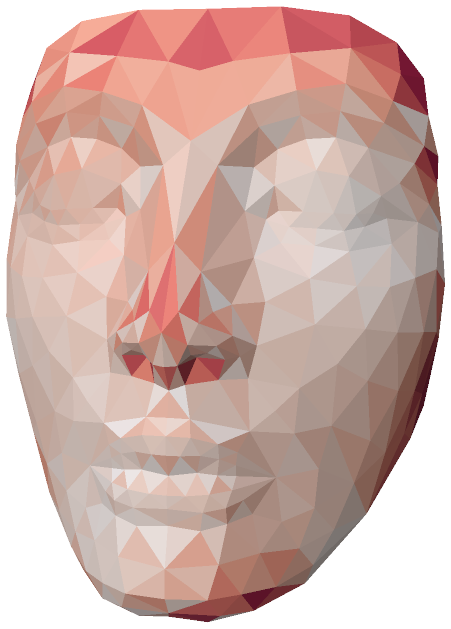
\includegraphics[width=\linewidth]{p2_nefertiti_arc_conf.png}\caption{\code{arc}}\end{subfigure}\quad
\begin{subfigure}{0.2\textwidth}\centering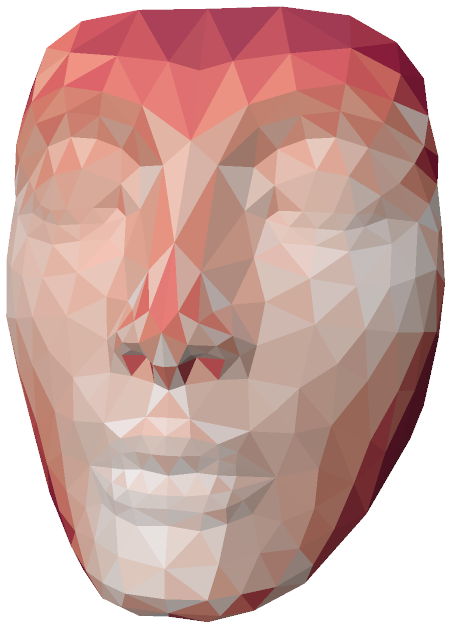
\includegraphics[width=\linewidth]{p2_nefertiti_uniform_conf.png}\caption{\code{uniform}}\end{subfigure}\quad
\begin{subfigure}{0.25\textwidth}\centering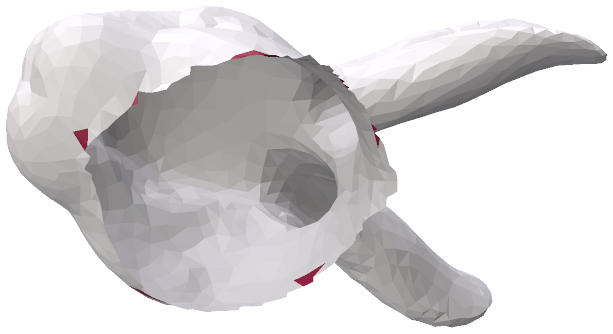
\includegraphics[width=\linewidth]{p2_bunny_estrella_3d.png}\caption{Bunny, estrella (\code{flips})}\end{subfigure}\quad
\begin{subfigure}{0.22\textwidth}\centering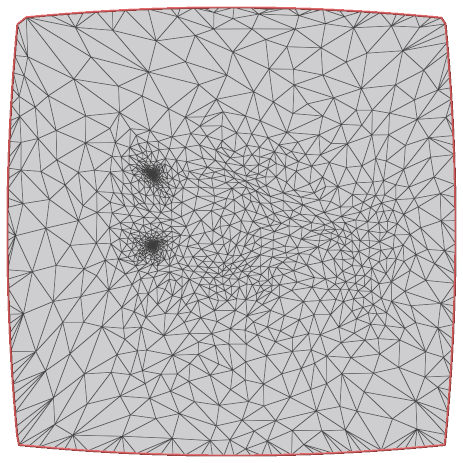
\includegraphics[width=\linewidth]{b1_bunny_uv.png}\caption{Bunny, \code{bulged\_square}}\end{subfigure}
\caption{(a, b) Distorsión conforme de Nefertiti (armónico, círculo) con cada espaciado: con \code{uniform} aumenta cerca del borde. (c) Caras invertidas con la estrella, junto al borde de la base. (d) Dominio con el cuadrado abombado del bonus B1.}
\end{figure}

\begin{table}[h]
\centering\small
\caption{Bonus B1: caras degeneradas (\code{degen}) con cada borde; entre paréntesis, cuántas tocan el borde.}
\begin{tabular}{llrrr}
\toprule
malla & pesos & \code{circle} & \code{square} & \code{bulged\_square} \\
\midrule
Nefertiti & uniform / harmonic / meanvalue & 0 / 0 / 0 & 0 / 0 / 0 & 0 / 0 / 0 \\
Bunny & uniform / harmonic / meanvalue & 0 / 0 / 0 & 4 (4) / 4 (4) / 4 (4) & 0 / 0 / 0 \\
Lucy & uniform & 184 (0) & 202 (23) & 179 (0) \\
Lucy & harmonic & 1\,418 (0) & 1\,442 (23) & 1\,419 (0) \\
Lucy & meanvalue & 978 (0) & 1\,008 (23) & 983 (0) \\
\bottomrule
\end{tabular}
\end{table}

\begin{figure}[h]
\centering
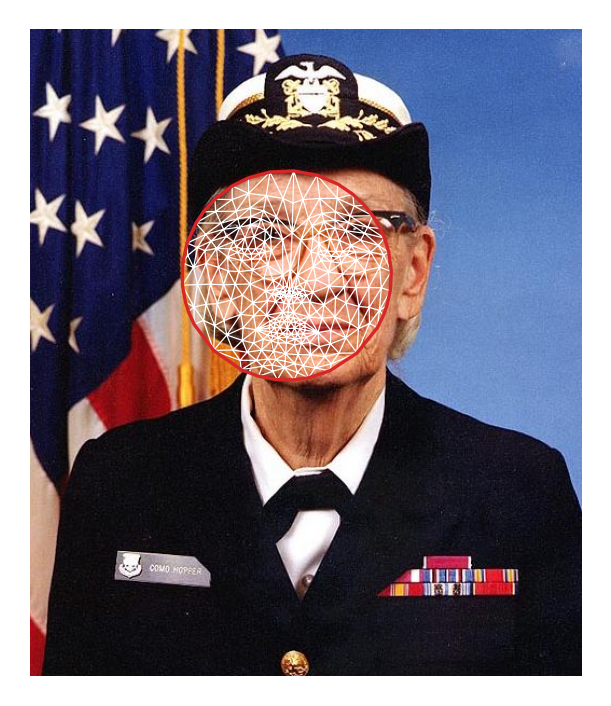
\includegraphics[height=4.2cm]{b2_harmonic_circle_uv.png}\quad
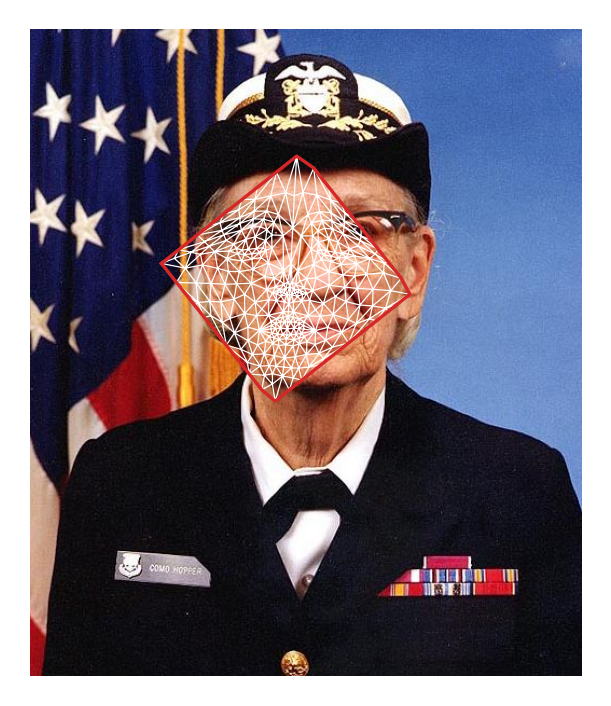
\includegraphics[height=4.2cm]{b2_meanvalue_square_uv.png}\quad
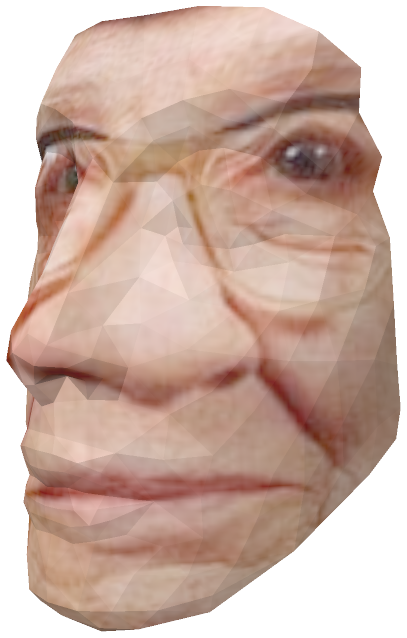
\includegraphics[height=4.2cm]{b2_harmonic_circle_lado.png}\quad
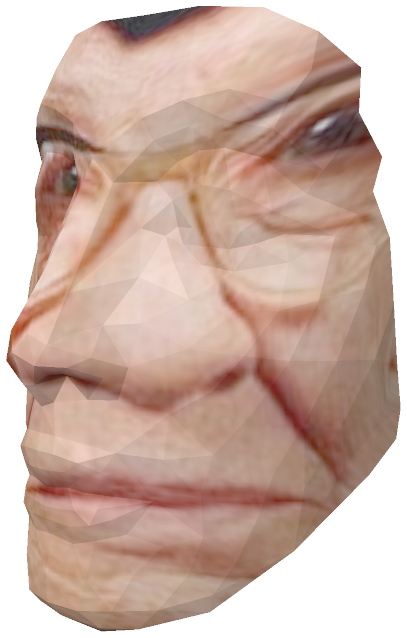
\includegraphics[height=4.2cm]{b2_meanvalue_square_lado.png}
\caption{Bonus B2: parte de la foto que usan armónico + círculo y valor medio + cuadrado, y sus vistas laterales.}
\end{figure}

\section{Reproducción de los resultados}\label{anx:reproduccion}
Desde \code{tarea3\_param/} (NumPy, SciPy, Polyscope y Matplotlib):
\begin{verbatim}
python tests.py                          # 12/12 pruebas
python experimentos/p1_pesos.py          # Parte 1
python experimentos/p2_bordes.py         # Parte 2 (y tablas --batch)
python experimentos/p3_lscm.py           # Parte 3
python experimentos/p4_distorsion.py     # Parte 4
python experimentos/p5_comparacion.py    # Parte 5
python experimentos/b1_cuadrado.py       # Bonus B1
python experimentos/b2_foto.py           # Bonus B2 y pregunta 5.3
python experimentos/tablas_latex.py      # tablas del Anexo A
\end{verbatim}
Las figuras y tablas (CSV) quedan en \code{experimentos/resultados/}; cada script imprime sus tablas (\code{log\_*.txt}).

\end{document}
